%-*-latex-*-

\begin{center}
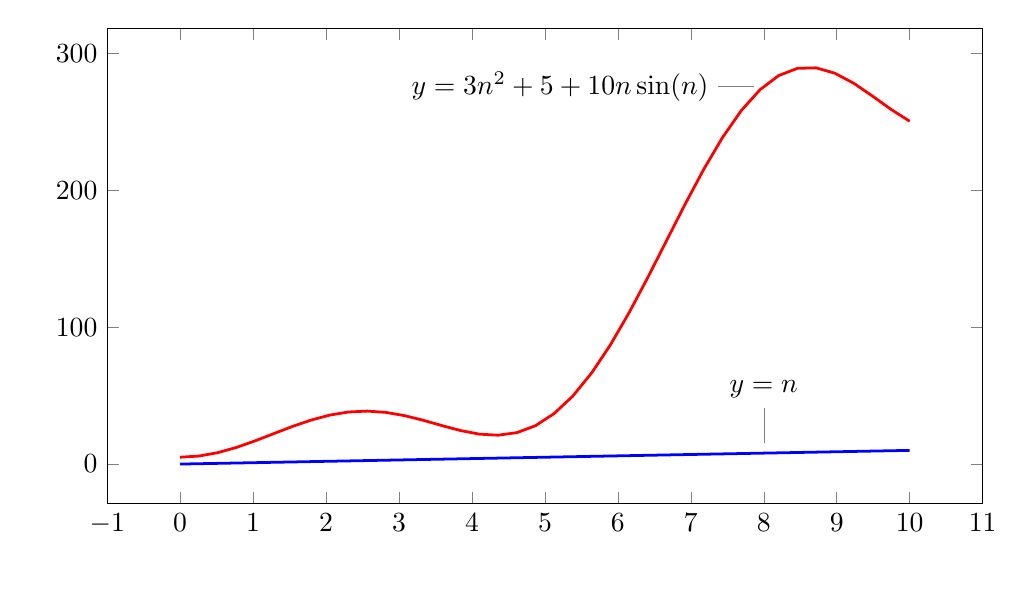
\begin{tikzpicture}[line width=1]
\begin{axis}[width=5in, height=3in,
             scatter/classes={a={mark=*,draw=black}},
             xlabel={\mbox{}},
             xlabel style={name=xlabel}, 
             ylabel={\mbox{}}, 
             legend style={
                at={(xlabel.south)},
                yshift=-1ex,
                anchor=north,
                legend cell align=left,
                },
        ]
]
\addplot[draw=red, line width=1] coordinates {(0.0,5.0)
(0.2564,5.8475)
(0.5128,8.305)
(0.7692,12.1258)
(1.0256,16.9255)
(1.2821,22.2207)
(1.5385,27.4772)
(1.7949,32.1647)
(2.0513,35.8134)
(2.3077,38.0661)
(2.5641,38.7219)
(2.8205,37.7672)
(3.0769,35.3908)
(3.3333,31.9811)
(3.5897,28.1044)
(3.8462,24.4672)
(4.1026,21.8624)
(4.359,21.1062)
(4.6154,22.9685)
(4.8718,28.1029)
(5.1282,36.9833)
(5.3846,49.851)
(5.641,66.6779)
(5.8974,87.1499)
(6.1538,110.6723)
(6.4103,136.3978)
(6.6667,163.2767)
(6.9231,190.1253)
(7.1795,215.7085)
(7.4359,238.832)
(7.6923,258.4347)
(7.9487,273.6771)
(8.2051,284.0168)
(8.4615,289.266)
(8.7179,289.6245)
(8.9744,285.6866)
(9.2308,278.4177)
(9.4872,269.1034)
(9.7436,259.2725)
(10.0,250.5979)
(10.0,250.5979)};\node[pin=left:{$y=3 n^2 + 5 + 10 n   \sin(n)$}] at (axis cs:8.0,276.14865972987053) {};\addplot[draw=blue, line width=1] coordinates {(0.0,0.0)
(5.0,5.0)
(10.0,10.0)
(10.0,10.0)};\node[pin=above:{$y=n$}] at (axis cs:8.0,8.0) {};
\end{axis}\end{tikzpicture}\end{center}
